\documentclass[11pt]{article}
\usepackage{sectsty}
\usepackage{enumerate}
\usepackage{bm}
\usepackage{amsmath, amsthm, amssymb}
\usepackage[usenames,dvipsnames]{color}
\usepackage{float, graphicx, nicefrac}
\usepackage{environ}
\usepackage{xeCJK}

\providecommand{\abs}[1]{\lvert#1\rvert}
\providecommand{\norm}[1]{\lVert#1\rVert}

\usepackage[sc]{mathpazo} % math & rm
\linespread{1.05}        % Palatino needs more leading (space between lines)
\usepackage[scaled=0.90]{helvet} % ss
% \usepackage[scaled=0.85]{sourcecodepro} % tt
\usepackage[T1]{fontenc}
\usepackage{textcomp}


\newtheorem{thm}{Theorem}
\newtheorem{lemma}[thm]{Lemma}
\newtheorem{fact}[thm]{Fact}
\newtheorem{cor}[thm]{Corollary}
\newtheorem{eg}{Example}
\newtheorem{ex}{Exercise}
\newtheorem{defi}{Definition}
\newtheorem{hw}{Problem}
\newenvironment{sol}
{\par\vspace{3mm}\noindent{\it Solution}.}
{\qed}

\newcommand{\ov}{\overline}
\newcommand{\cb}{{\cal B}}
\newcommand{\cc}{{\cal C}}
\newcommand{\cd}{{\cal D}}
\newcommand{\ce}{{\cal E}}
\newcommand{\cf}{{\cal F}}
\newcommand{\ch}{{\cal H}}
\newcommand{\cl}{{\cal L}}
\newcommand{\cm}{{\cal M}}
\newcommand{\cp}{{\cal P}}
\newcommand{\cz}{{\cal Z}}
\newcommand{\eps}{\varepsilon}
\newcommand{\ra}{\rightarrow}
\newcommand{\la}{\leftarrow}
\newcommand{\Ra}{\Rightarrow}
\newcommand{\dist}{\mbox{\rm dist}}
\newcommand{\bn}{{\mathbf N}}

\newcommand{\bA}{ \bm{A} }
\newcommand{\bI}{ \bm{I} }
\newcommand{\bM}{ \bm{M} }
\newcommand{\bx}{ \bm{x} }
\newcommand{\bV}{ \bm{V} }
\newcommand{\bC}{ \bm{C} }
\newcommand{\bc}{ \bm{c} }
\newcommand{\bU}{ \bm{U} }
\newcommand{\bR}{ \bm{R} }
\newcommand{\bW}{ \bm{W} }
\newcommand{\bX}{ \bm{X} }
\newcommand{\bY}{ \bm{Y} }
\newcommand{\bZ}{ \bm{Z} }
\newcommand{\br}{ \bm{r} }

\newcommand{\onef}[1]{ \nicefrac{1}{#1} }
% \setlength{\parindent}{0pt}
% \setlength{\parskip}{2ex}
% \newenvironment{proofof}[1]{\bigskip\noindent{\itshape #1. }}{\hfill$\Box$\medskip}

\usepackage{enumerate,fullpage,proof,color,hyperref}


\newcommand{\todo}[1] { \color{red}[TODO: #1]\color{black} }


\newcommand{\alns}[1] {
	\begin{align*} #1 \end{align*}
}
\newcommand{\pd}[2] {
  \frac{\partial #1}{\partial #2}
}

\title{Big Data Processing: homework 7}
\author{凌康伟 \qquad 5140219295}

\begin{document}
\maketitle

\section*{Exercise 1}
The stochastic adjacency matrix:
\[
  \bM =
  \begin{bmatrix}
    0 & \onef{3} & 1 \\
    1 & \onef{3} & 0 \\
    0 & \onef{3} & 0
  \end{bmatrix}
\]
Solve for the equation: $\bM \lambda = \lambda$ (with $r_1 + r_2 + r_3 = 1$):
\[
  \begin{bmatrix}
    r_1 \\ r_2 \\ r_3
  \end{bmatrix}
  =
  \begin{bmatrix}
    \onef{3} \\ \onef{2} \\ \onef{6}
  \end{bmatrix}
\]

\section*{Exercise 2}
\begin{enumerate}[1.]
\item
  \[
    \bM =
    \begin{bmatrix}
      \onef{3} & \onef{2} & 0        & 0\\
      0        & 0        & \onef{2} & 1\\
      \onef{3} & 0        & 0        & 0\\
      \onef{3} & \onef{2} & \onef{2} & 0
    \end{bmatrix}
  \]
\item
  \[
    \bA = \beta \bM + (1 - \beta)[\dfrac{1}{4}]_{4\times 4} =
    \begin{bmatrix}
      0.325 & 0.475 & 0.025 & 0.025\\
      0.025 & 0.025 & 0.475 & 0.925\\
      0.325 & 0.025 & 0.025 & 0.025\\
      0.325 & 0.475 & 0.475 & 0.025
    \end{bmatrix}
  \]
\item Initial value:
  \[
    \br^0 =
    \begin{bmatrix}
      \onef{4} \\ \onef{4} \\ \onef{4} \\ \onef{4}
    \end{bmatrix}
  \]
  one iteration:
  \[
    \br^1 = \bA \br^0 =
    \begin{bmatrix}
      0.2125 \\ 0.3625 \\ 0.1 \\ 0.325
    \end{bmatrix}
  \]
\end{enumerate}
\section*{Exercise 3}
Perfect matchings:
\begin{center}
  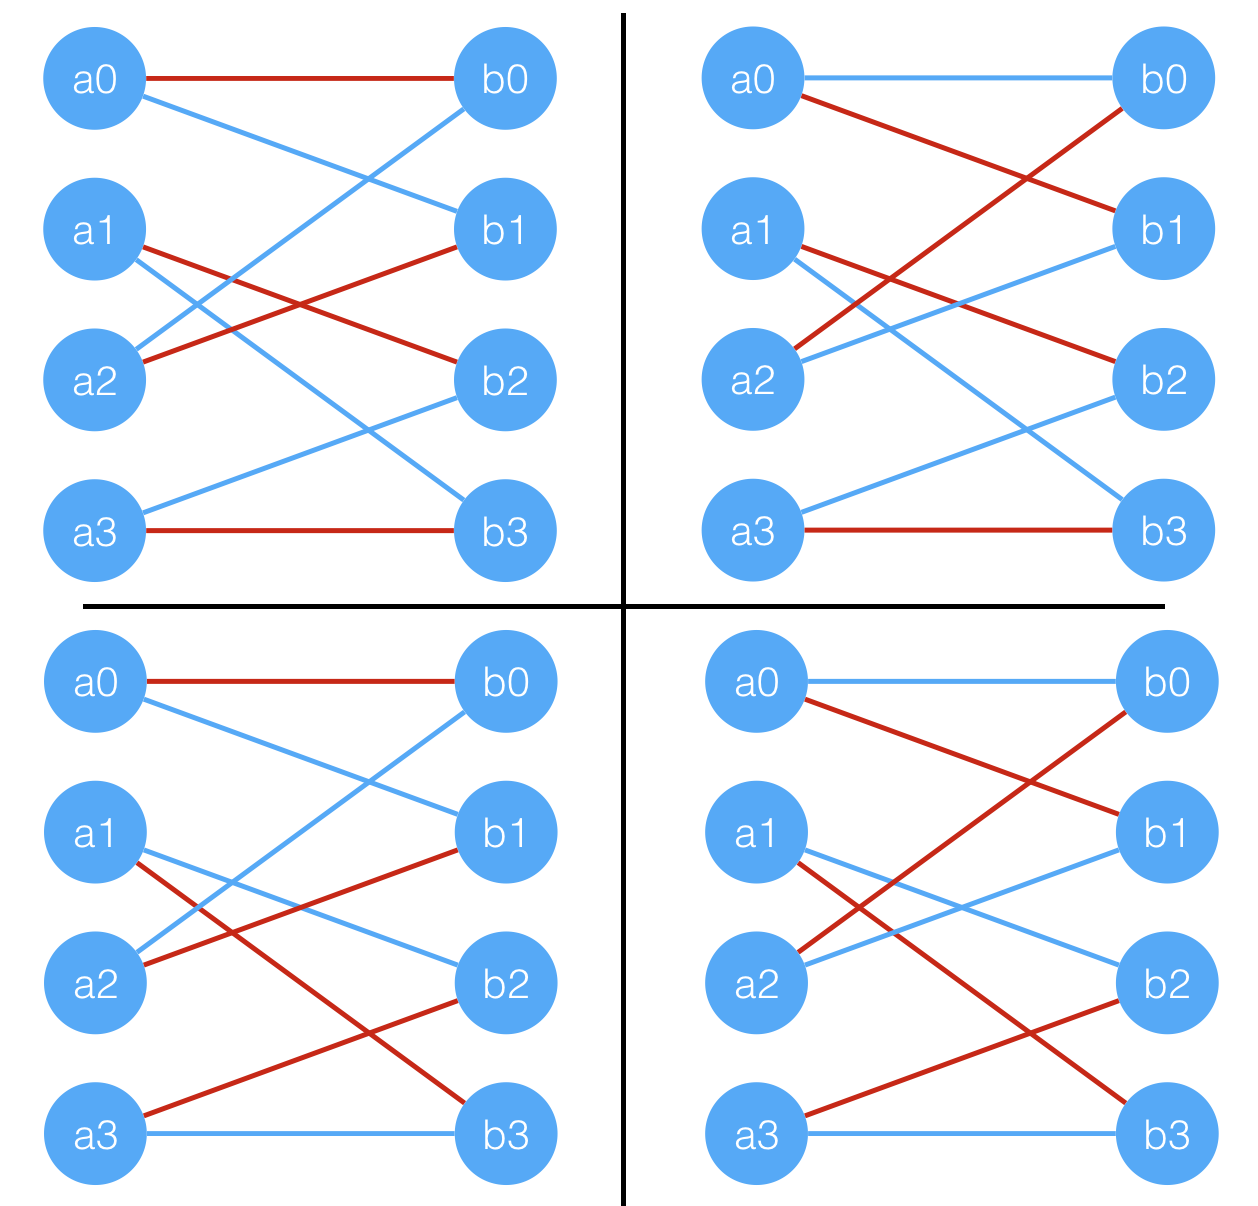
\includegraphics[width=\linewidth]{matchings.png}
\end{center}
\end{document}